\section{資訊檢索與語音資訊檢索}

\subsection{資訊檢索}


資訊檢索 (Information Retrieval,IR)
是指從資料庫中擷取出與某個主題(Topic)相關之檢索對象(Object)的行為。基本使用流程為:使用者輸入了一段查詢對象 $ Q $ (Query),系統能夠從資料庫中傳回和這個主題相關的檢索對象(Object),並進一步依據檢索對象和主題的相關程度進行排序(Ranking),以方便使用者瀏覽並取得所需的檢索對象。如圖\ref{fig:ch2_IR}。
\begin{figure}
\centering
\includegraphics[scale=0.4]{images/ch2_Ir.png}
\caption{資訊檢索系統基本架構} \label{fig:ch2_IR}
\end{figure}

檢索對象  $ x $ 
指的是系統所檢索出的東西,例如:在文字搜尋中檢索對象指的是文章、在網路檢索中指的是網頁、在圖像檢索指的是圖片、在語音檢索指的是口語片段(Spoken Segment)等,同時,查詞對象  $ Q $  也可以為圖片、文字或聲音。
本篇論文中所使用的查詢詞  $ Q $  形式有二:文字構成的字串、口述形式。本篇論文使用  $ x $  則都是語音文件。

當有了查詢對象,系統的主要任務就是去計算相關性(Relevance),其定義為  $ P(R|x,Q) $  ,然後依此機率大小對檢索對象進行排序,這個排序方式
被稱為機率排序原則 (Probability Ranking Principle,PRP)\cite{robertson1997probability}。
這個相關性函式通常是按照檢索系統的需求去決定的,可以是用機器學習(Machine
learning)的方法學習出來,也可以是由系統設計者決定。上述的方法可以視為一個分類問題(Classfication),另一種方法為排序學習(Learning
to Rank),此時系統不在需要計算  $ P(R|x,Q) $ ,而是尋找一個排序函式(Ranking Function)
 $ S(x,Q) $ ,能夠將 $  S(x_T,Q)>s(x_F,Q) $ ,  $ x_T $  為相關的檢索對象、  $ x_F $ 
為不相關的檢索對象。也就是說,所有相關的檢索對象,都能夠超過不相關的檢索對象。

如何檢驗一個資訊系統的好壞也是重要的課題首先我們必須要準備測試集,其中包含文件資料庫、查詢詞、以及與每個查詢詞對應的相關文件的標註。藉由評估系統在測試集上於「正確度」、「速度」、以及「佔用空間」等數個面向的表現,以了解此系統與其他系統的優劣比較。

文字檢索會議 (The Text REtrieval Conference,TREC),自1992年起每年的居舉行會議,並在多個測試項目上提供大規模之標準測試集,藉此讓來自世界各地的參加團隊評估自己的系統效益同時與其他團隊相互討論切磋。如今,TREC除英文的檢索測試集外,更提供了非英文的大規模檢索測試集
(如西班牙文與中文)、語音檢索測試集、以及跨語言檢索測試集。另外在測試項目上也有了多樣的發展,包括引入了開放領域自動問答
(Open-Domain Question Answering)以及基於內容的數位影音檢索
(Content-based Retrieval of Digital Video)
等。資訊檢索已是一門受到關注的領域。



\subsection{語音資訊檢索}
目前語音檢索可以分為兩類,「口述語彙偵測 (Spoken Term
Detection)」與「語意檢索 (Semantic
Retrieval)」,本論文著重在口述詞彙偵測,在此將兩者簡介如下:

\subsubsection{口述語彙偵測}


口述語彙偵測的目的是檢索出所有包含查詢詞的語音文件,著重於逐詞比對(Literal
Term
Matching),主要有兩種檢索情境。第一種是先將語音文件辨識為詞圖(Lattice)後,當使用者輸入文字的查詢詞後,系統會在詞圖上進行查詢詞的檢索。這種檢索情境需要有訓練好的自動語音辨識系統(Automatic Speech Recognition,ASR),由於語音辨識系統並無法保證在所有情況下都有很好的辨識率,因此由辨識錯誤所導致的檢索性能下降是在此最需要解決的問題。過去的文獻有用聲學特徵如梅爾倒頻譜係數
(Mel-Frequency Cepstral Coefficients (MFCC))幫助分類器 (Classifier)
在分類一篇語音文件是否相關時的判斷,也有利用相關回饋 (Relevance Feedback)、圖論 (Graph)與隨機漫步 (Random Walk)
解決這些問題。

第二種是非監督式
(Unsupervised),的方法,查詢詞與語音文件都是語音形式的,也有人稱之為依例查詢
(Query-by-Example),系統直接利用如動態時間校準(Dynamic Time Warping)
等方法在信號上比對語音文件中是否有某一段聲音與查詢詞很相像,過去的方法通常是為了解決不同文件間語速上的差異提出如有斜率限制的動態時間校準(Slope-Constraint
DTW),或是為了解決動態時間校準逐一比對所有文件庫所花時間過多的問題。計算此情境下的
 $ S(Q, x) $  為利用片段式動態時間規劃 (Segmental Dynamic Time Warping),簡介於~\ref{sec:chap4_sdtw}。

\subsubsection{語意檢索}
語意檢索的目的為回傳概念上相關的語音文件,而不一定要出現查詢詞。希望查詢結果與輸入的查詢詞是概念上匹配(Concept
Matching)的,而不是只回傳有出現查詢詞的文件,如當使用者查詢「美國總統」,文件中包含「美國總統」、「美國白宮」,而不是與查詢詞完全一樣的文件,通常也是使用者想要的。文字領域的資訊檢索已經有「概念匹配」的做法來達到語意檢索,但是由於文字領域的資訊檢索是在文字為完全正確的狀況下,不像語音數位文件的檢索往往會有辨識錯誤的問題。對於語音文件,一個較常見的實作方法通常是使用相關回饋(Relevance Feedback)~\cite{ruthven2003survey} 與查詢詞擴展(Query Expansion)~\cite{voorhees1994query,xu1996query}。

\subsection{片段式動態時間校準 (Segmental DTW)}
\label{sec:chap4_sdtw}
口述語彙偵測的目的為搜尋整個語料庫後,找出其中有出現查詢詞的語音文件,同時找出這些語音文件中可能有出現查詢詞的假設區域 (Hypothesized Region) ,並給這個假設區域一個相關分數,最後系統再根據相關分數進行排序後回傳給使用者 (分數較高為較相關)。

這裡考慮的口述語彙偵測是查詢詞也是語音形式的情境。此時所用的方法為片段式動態時間校準 (Segmental Dynamic Time Warping)~\cite{chan2010unsupervised, hazen2009query}。假設輸入的查詢詞的特徵為 $ \mathbf{X} = (\mathbf{x}_1, ..., \mathbf{x}_{|\mathbf{X}|}) $ ,語音文件的特徵為 $ \mathbf{Y} = (\mathbf{y}_1, ..., \mathbf{y}_{|\mathbf{Y}|}) $ ,有了這兩者之後,就可以建立一個距離表格 (Distance Table)  $ D(i, j) = \rho(\mathbf{x}_i, \mathbf{y}_j) $ ,通常這裡使用的特徵是
高斯事後機率 (Gaussian Posteriorgrams)~\cite{zhang2009unsupervised}或是梅爾倒頻譜係數
(MFCC)。如果使用高斯事後機率的話,兩個音框之間的距離為
 $ \rho(\mathbf{x}_i, \mathbf{y}_j) \equiv -\log (\mathbf{x}_i
\cdot\mathbf{y}_j) $ 。如果使用梅爾倒頻譜係數的話,兩個音框之間的距離為兩點之間的歐幾里得距離(Euclidean
Distance),即 $ \rho(\mathbf{x}_i, \mathbf{y}_j)
\equiv\sqrt{|\mathbf{x}_i - \mathbf{y}_j|^2} $ 。

動態時間校準的目的是要在  $ D(i, j) $  上找一條距離總合最短的路徑從  $ (1, s) $  到  $ (|\mathbf{X}|, e) $  表示從  $ \mathbf{X} $ 對應到 $ (\mathbf{y}_s, ..., \mathbf{y}_e) $  (因為查詢詞一定要被完全對應,而語音文件不一定要被完全對應到)。由於假設區域可以出現在語音文件中的任何地方, 因此片段式動態時間校準將距離表格  $ D(i, j) $  切成數個重疊的對角片段 (寬度為  $ R $ ),所以說每個片段的起始點分別為  $ (1, 1), (1, 1+R), (1, 1+2R),... $  如圖 ~\ref{fig:chap4_sdtw} 所示,每個對角片段都代表了一個可能出現查詢詞的區域,所以要在每個對角片段上找出距離總合最短的路徑,即這個對角片段上的假設區域。片段式動態時間校準會從每個片段中找出一段距離總合最短的路徑,在每個片段中所有對應的路徑 (Warping Path) 都必須要完整地待在片段內,不可超出片段。

\begin{figure}[h]
\centering
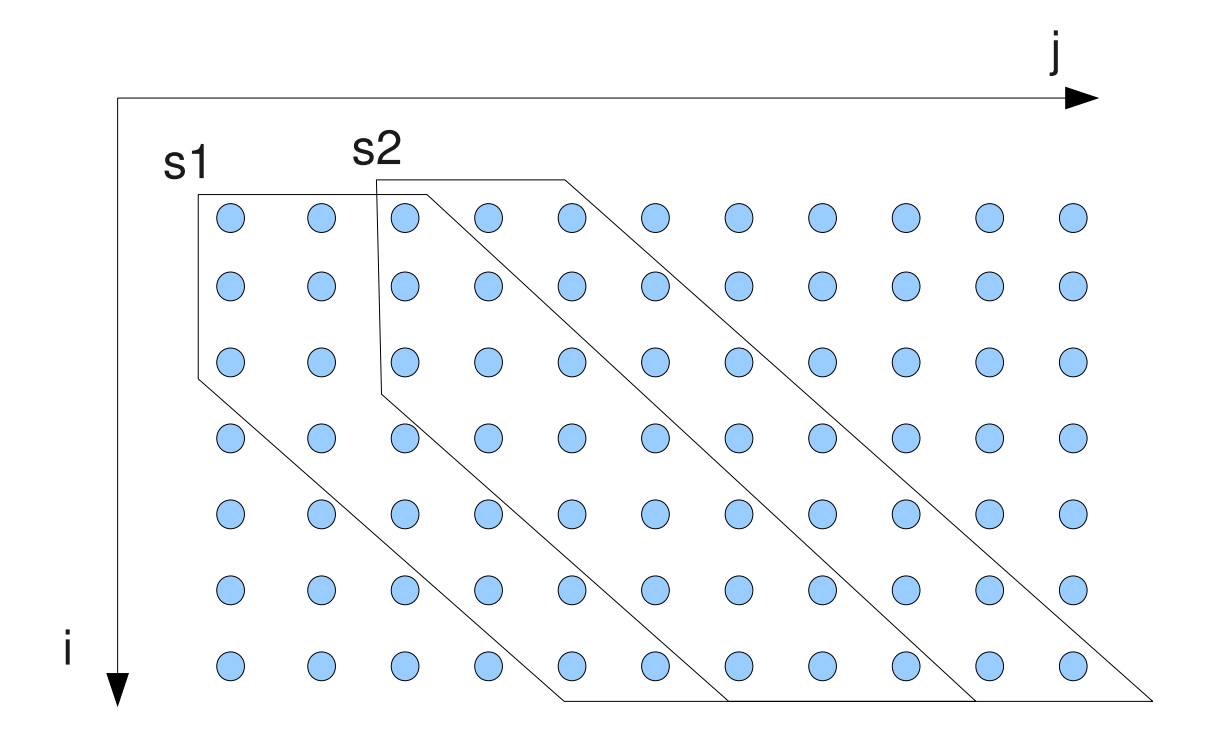
\includegraphics[scale=0.3]{images/chap4_sdtw.png}
\caption{片段式動態時間校準示意圖~\cite{zhang2009unsupervised}} \label{fig:chap4_sdtw}
\end{figure}

假設在每個片段中的對應路徑為:

\[
\phi = (i_t, j_t), t = 1,...,|\phi|
\]

代表著如下的對應關係:

\[
\mathbf{x}_{i_1} \leftrightarrow \mathbf{y}_{j_1}, \mathbf{x}_{i_2} \leftrightarrow \mathbf{y}_{j_2},...,\mathbf{x}_{|\phi|} \leftrightarrow \mathbf{y}_{|\phi|},
\]
而邊界條件是  $ i_1 = 1, i_{|\phi|} = |\mathbf{X}| $  , $ j_1 $  為  $ 1+kR $  ,對應路徑中所有的點都要在片段內,即:

\[
|(i_t-i_1)-(j_t-j_1)| <= R
\]

而片段式動態時間校準的目標是要在每個片段內找到一條路徑  $ \phi $  使得下式的距離總和最小:

\begin{equation}
C_{\phi}(\mathbf{X}, \mathbf{Y}) = \sum_{t=1}^{|\phi|} \rho(\mathbf{x}_{i_t},\mathbf{y}_{j_t})
\end{equation}

\begin{figure}[h]
\centering
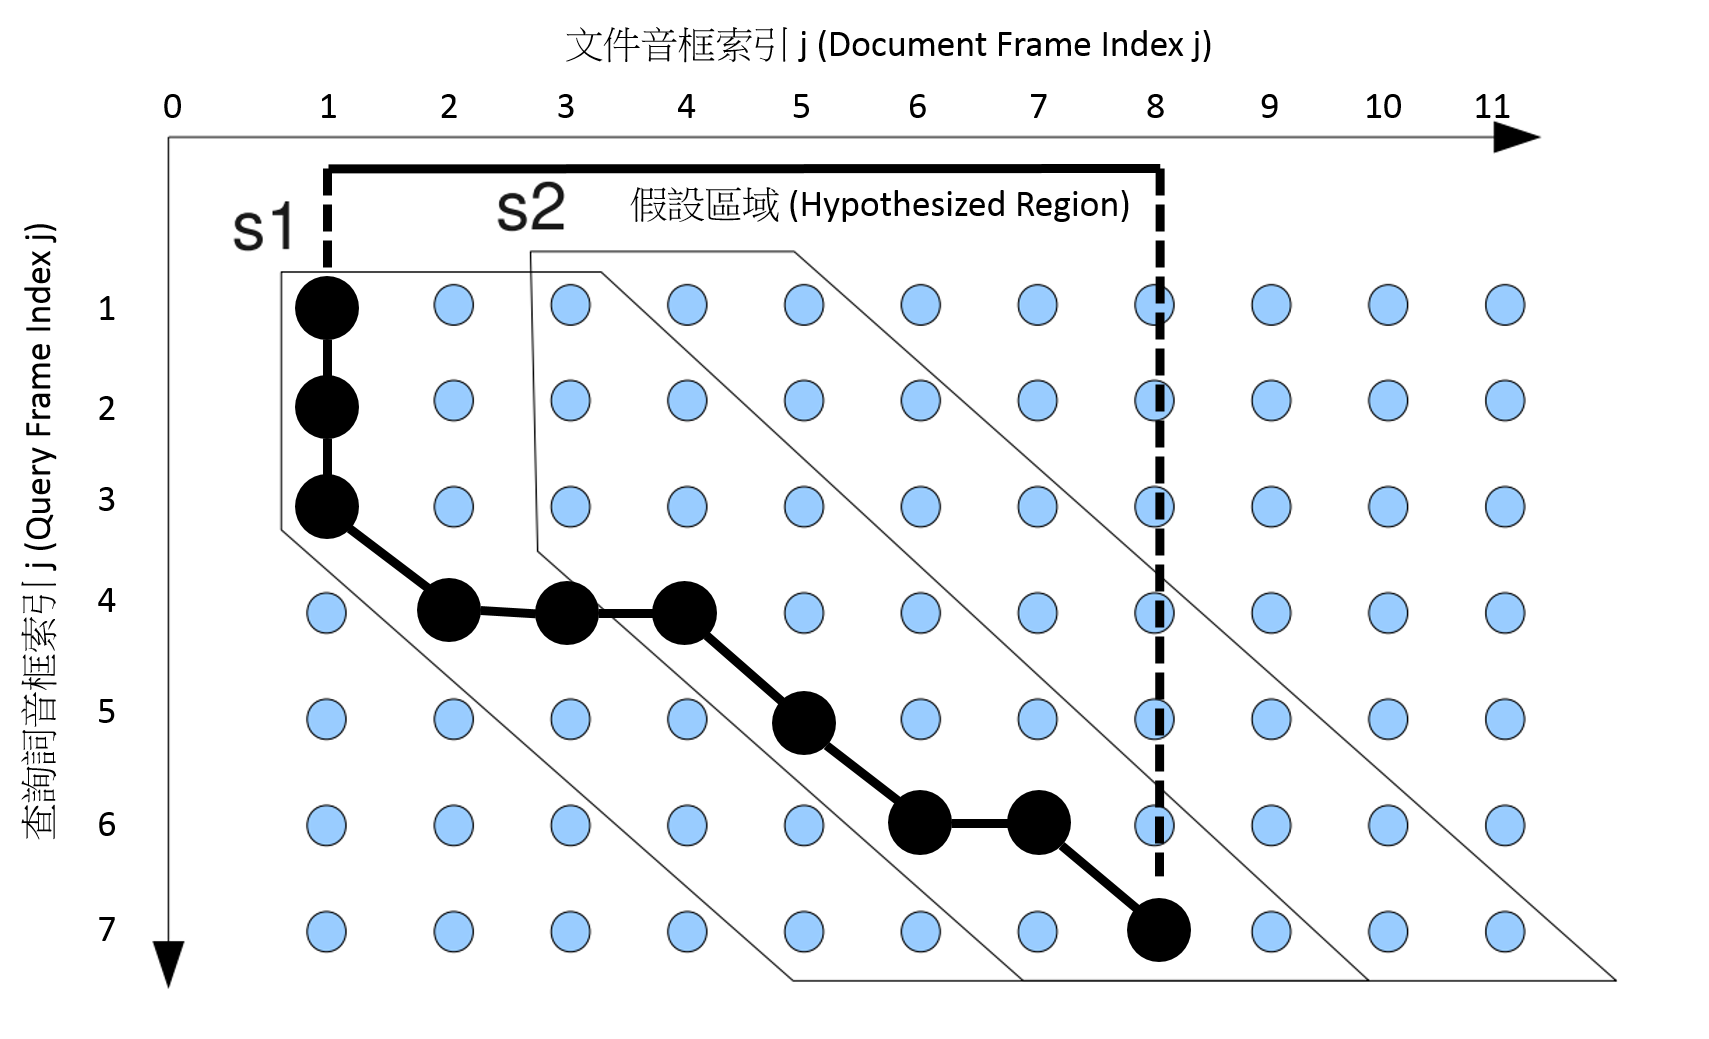
\includegraphics[scale=0.4]{images/chap2_segdtw_exp1.png}
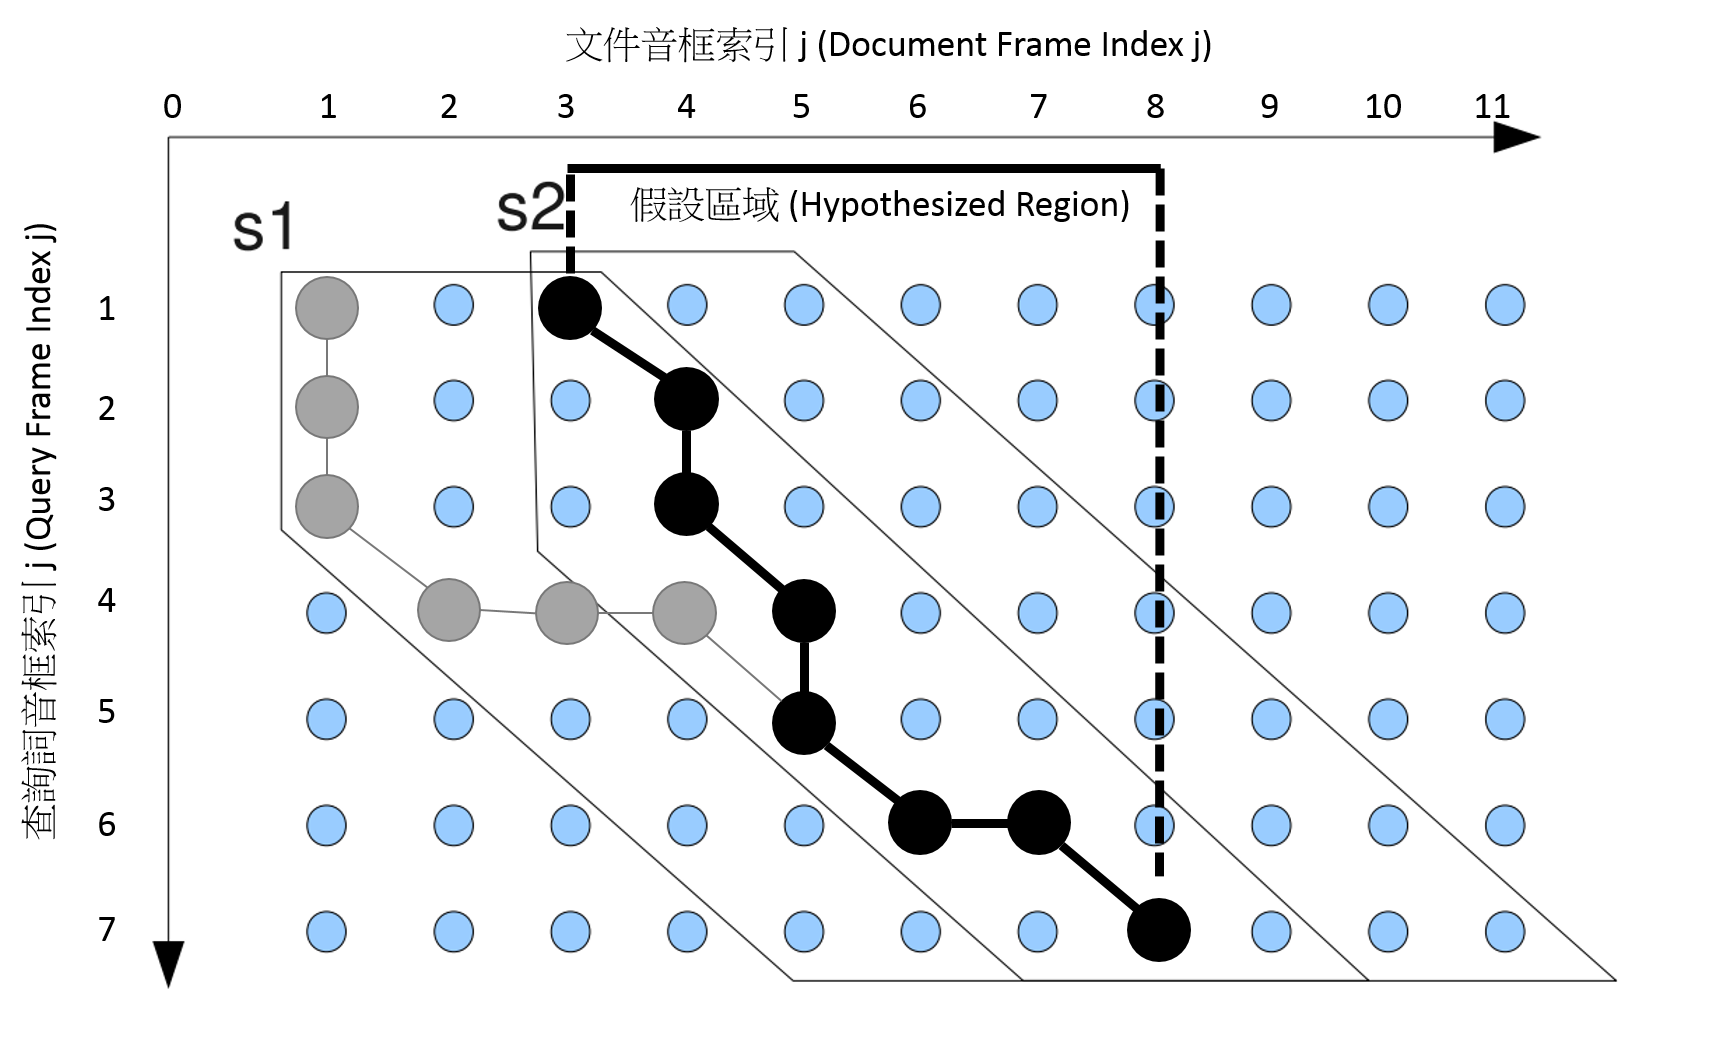
\includegraphics[scale=0.4]{images/chap2_segdtw_exp2.png}
\caption{示意如何從兩個對角片段中找到相關分數最大的假設區域,其中  $ R=2 $ }
\label{fig:chap2_sdtw_exp}
\end{figure}




每個片段中使得  $ C_{\phi}(\mathbf{X}, \mathbf{Y}) $  最小,即使得相關分數  $ -C_{\phi}(\mathbf{X}, \mathbf{Y}) $  最大的那條  $ \phi $  即為每個片段中的假設區域  $ (\mathbf{y}_{j_1},...,\mathbf{y}_{j_{|\phi|}}) $  ,而在每個片段中找到最大相關分數的路徑可以使用動態規劃 (Dynamic Programming) 求解。圖~\ref{fig:chap2_sdtw_exp}中顯示了兩個對角片段與其對應的最大相關分數的路徑與假設區域。圖中上半部中的  $ (\mathbf{y}_1, ..., \mathbf{y}_8) $  代表在第一個對角片段中找到的假設區間,圖中下半部中的  $ (\mathbf{y}_3, ..., \mathbf{y}_8) $  則是在第二個對角片段中找到的假設區域。 找到所有假設區域後,將假設區域按照其與查詢詞的相關分數進行排序後,即為口述語彙偵測的結果。在一篇語音文件中找到所有可能的假設區域需要  $ O(|\mathbf{X}||\mathbf{Y}|) $  的計算量來計算點與點之間的距離  $ \rho $ ,並需要 $ O(|\mathbf{X}||\mathbf{Y}|) $ 的計算量來找到相關分數最大的路徑。

\vspace{20mm}
\subsection{資訊檢索評估機制}
為了有效比較彼此系統,制訊檢索評估機制的標準是很重要的一環,本節將對一些常見以及本論文所使用的評分標準一一做介紹。

\subsubsection{準確率(Precision)與召回率(Recall)}
檢索系統找出的所有可能相關檢索對象中,真正相關的比例稱之為準確率,準確率高代表所找出的檢索結果的可信度高;
而所有真正的相關檢索對象有多少比例被系統檢索出來,我們稱之為召回率,召回率高代表系統找回越多相關的檢索目標。通常會為系統設定一個閥值(Threshold),文件的分數若高於閥值,則視為相關,反之若文件的分數低於閥值,則視為不相關。準確率和召回率的定義如下:

\[
\text{準確率}=\frac{\text{檢索到的相關檢索對象數}}{\text{檢索到的檢索對象數}}
\]

\[
\text{召回率}=\frac{\text{檢索到的相關檢索對象數}}{\text{所有的相關檢索對象數}}
\]

通常這兩個值彼此之間的關係為負相關。調高閥值的話準確率會上升,但召回率則會下降;反之若調低閥值,準確率會因此下降,召回率則會很高。可以考慮一個極端例子:當閥值非常低時,幾乎所有的文件都是相關文件,此時的召回率相當於1,但準確率就會很低了。因此單看準確率或召回率是無法準確地評估系統的優劣的,必須要兩者一起評估。

\begin{figure}
\centering
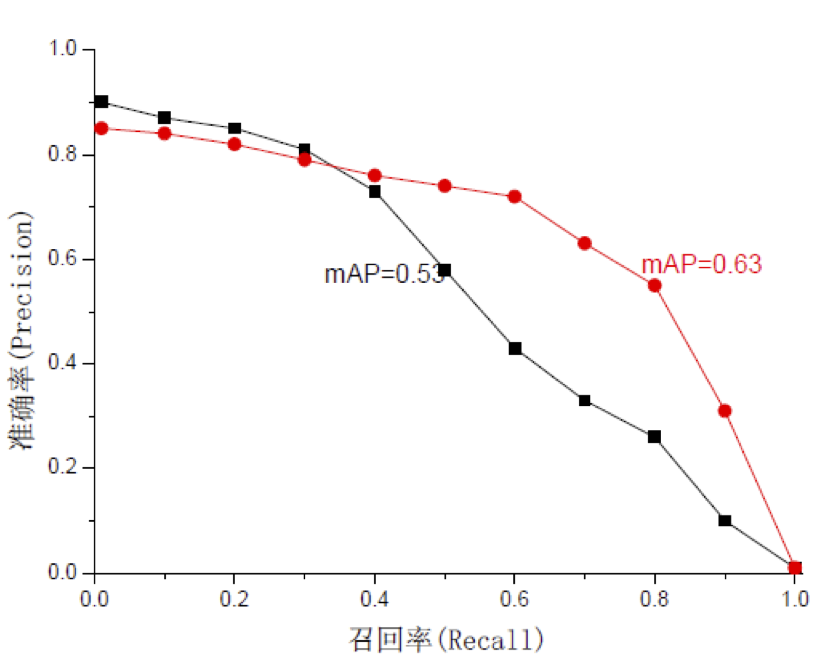
\includegraphics[scale=0.5]{images/chap2_precision_recall.png}
\caption{準確率、召回率和平均準確率之關係} \label{fig:precision_recall}
\end{figure}

\subsubsection{P@N}

通常使用者最重視的是檢索系統傳回的前幾名結果,所以就發展出了 $ P@N $ 這個評估機制。 $ P@N $ 就是只看前N個檢索結果的正確率。例如:前五個檢索結果中有一個是相關的,那 $ P@5 $ 就是20\%。

 $ P@N $ 的定義如下:
\[
P@N=\frac{\text{前N個文件裡的相關文件數}}{N}
\]
 然而由於不同的查詢詞其相關的檢索對象數不同,因此  $ P@N $  有時候並非公平的評比方式, 舉
 例來說,如果整個資料庫裡面相關的檢索對象只有5個,  $ P@10 $  最高就只能到
 0.5。
\subsubsection{平均準確率~\cite{garofolo2000trec}}

因為準確率和 $ P@N $ 都需要事先決定,當查詢詞和條件不同時,很難準確地評估兩個系統的效能。因此有人提出了平均準確率(Mean Average Precision, MAP)的概念,如圖~\ref{fig:precision_recall},平均準確率就是準確率和召回率曲線下面積的平均值。平均準確率的定義如下:
\begin{equation}
MAP = \frac{1}{|Q|} \sum_Q \frac{\sum_{d \in D^R}precision(d)}{|D^R|}
\end{equation}
其中Q代表查詢詞的集合, $ |Q| $ 為查詢詞的總數, $ D^R $ 為和查詢詞Q相關的文件d的集合, $ |D^R| $ 代表和查詢詞Q相關的文件數量。precision(d)代表系統檢索出文件d時的準確率。




\section{深層類神經網路(Deep Neural Network, DNN)}
\label{DNN}
\subsection{簡介}
深層類神經網路發想於生物的神經系統結構。神經系統由非常多的神經元組成,彼此以樹突、軸突與突觸連結,每顆神經元自己有活化閾值來決定激發
態與否。根據此仿生的觀察,便產生一種數學模型(如圖~\ref{fig:ch2_bio_neuron}與~\ref{fig:ch2_math_neuron}),將其層層疊起(如圖~\ref{fig:ch2_DNN}),即為深度類神經網路的全貌。
\begin{figure}[hb]
\centering
\subfloat[][生物學上的單顆神經元結構]{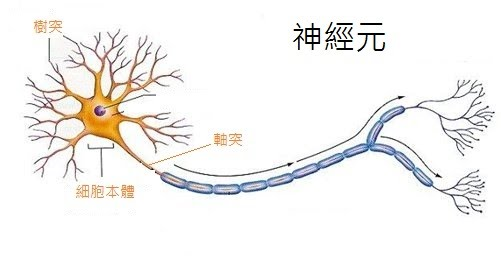
\includegraphics[scale=0.3]{images/ch2_bio_neuron.jpg}\label{fig:ch2_bio_neuron}}
\subfloat[][數學上的單顆神經元結構(感知器)]{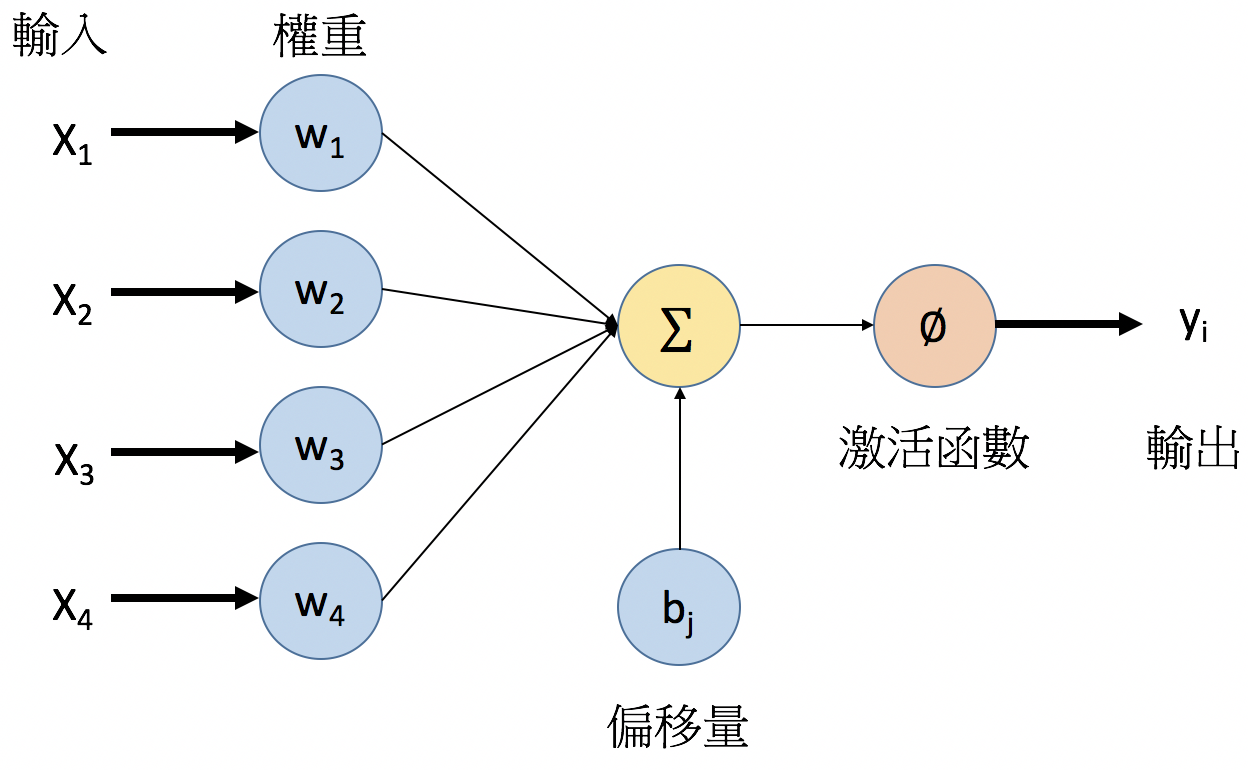
\includegraphics[scale=0.3]{images/ch2_single_neuron.png}\label{fig:ch2_math_neuron}}
\caption{類神經網路的單顆神經元}
\end{figure}

\begin{figure}[h]
\centering
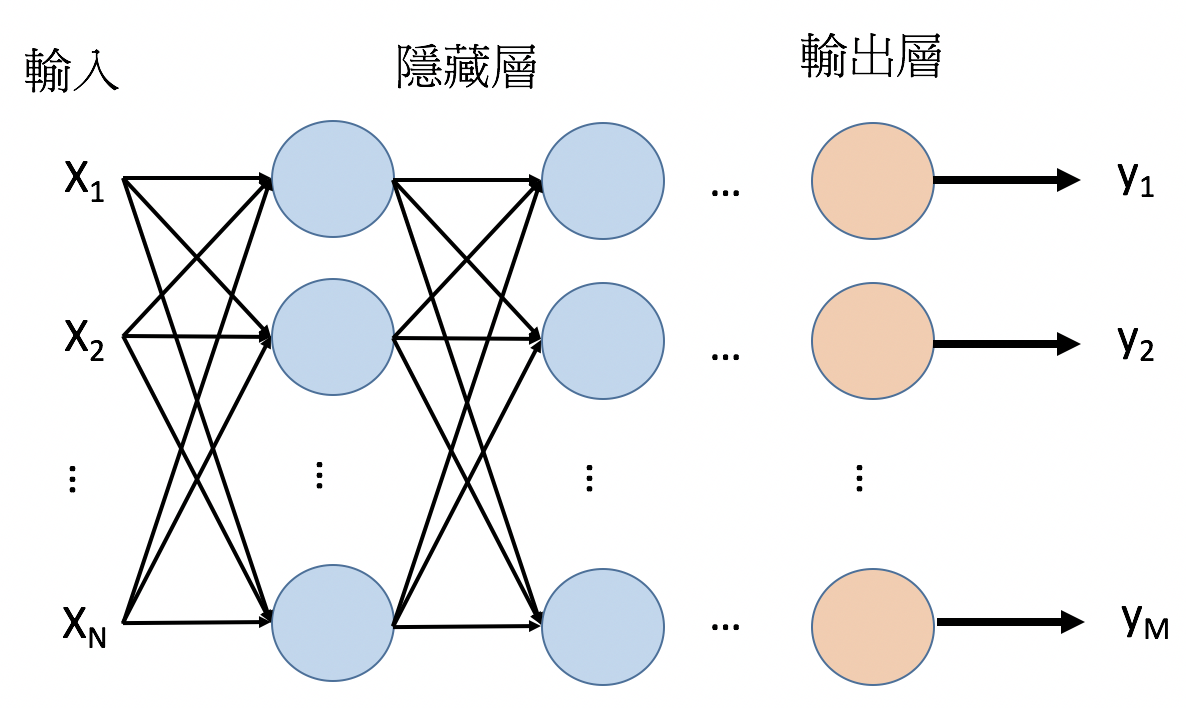
\includegraphics[scale=0.3]{images/ch2_DNN.png}
\caption{基本深度類神經網路架構圖} \label{fig:ch2_DNN}
\end{figure}

深度類神經網路是目前機器學習重要的一個分支,曾經在1980年代蓬勃發展,但因計算代價太高,且同時有其他簡單的模型如支撐向量機(Support
Vector Machine)的興起而沒落。深層學習的概念由辛氏(Geoffrey Hinton)於2006重新推出~\cite{hinton2006fast},並使用一種新型的訓練方法,能夠有效提升訓練的執行速度;加上圖形處理器(Graphics
Processing
Unit,GPU)大幅提高了數值和矩陣運算的速度,使得深層類神經網路重新成為機器學習領域中的重要角色。
\subsection{運作原理}
類神經網路的架構如圖~\ref{fig:ch2_DNN},其結構由感知器(Perceptron)~圖\ref{fig:ch2_math_neuron}串接而成,因此深層類神經網路又稱為多層感知器(Multi-layer
Perceptron,MLP)。每一層根據所在位置可分為三類:
\begin{itemize}
\item    輸入層(Input Layer): 即為類神經網路輸入特徵向量(Feature Vector) $ \bold{X} = [x_1 , x_2 , x_3 , x_4 ... , x_N]^T $ 
\item    隱藏層(Hidden Layer): 類神經網路的主要部分,可以有很多層,且每層的感知器(神經元)數目可以不同。
\item    輸出層(Output Layer): 跟隱藏層很相似,不過會依據模型的目的有所改變。譬如回歸問題,此時輸出層就不會經過活化函數。對於分類問題,輸出層的數量會跟標記種類(Class)相同。
\end{itemize}

每個感知器都包含了一組加權係數跟偏移量(Bias),跟非線性的活化函數(Activation
Function)。數學式如下:
\begin{equation}
	y_i = \phi{(\sum_{i=1}^{M} w_{ij}x_i+b_j) }
\end{equation}

其中 $ \phi $ 是活化函數, $ w_{ij} $ 是第 $ j $ 個感知器中,對應到第 $ i $ 個輸入 $ x_i $ 的加權係數, $ b_j $ 是第 $ j $ 個感知器的偏移量。 $ \phi $ 括號內的特徵轉換稱為仿射變換(Affine
Transformation)。可將之想像為一個從 $ M $ 維實數空間映射到 $ N $ 維實數空間的函數 $ A:
R^M \rightarrow R^N $ ,其中 $ M $ 和 $ N $ 分別是輸入向量 $ x $ 與輸出向量 $ y $ 的維度。由於仿
射變換可看成是一個線性矩陣的轉換,複雜度並不夠高,因此我們引入 $ \phi $ 這個非線性的活化函數。常見的活化函數分別為S型函數(Sigmoid)和整流線性單元(Rectified Linear Unit, ReLU)。
\begin{equation}
\begin{aligned}
&sigmoid(x) = \frac{1}{1 + e^{-x}}
\\
&ReLU(x) = max( 0 , x )
\end{aligned}
\end{equation}


\subsection{訓練類神經網路}
\label{ch2_train_DNN}
深層類神經網路常見的訓練方法為反向傳播演算法(Back
Propagation)\cite{rumelhart1988learning},通常要搭配一些最佳化演算法(Optimization
Method)例如梯度下降法(Gradient Descent)。
其概念為模型會計算出當下錯誤的程度,並依照可以減少錯誤的方向更改參數。為了定義錯誤的程度,需借用到損失函數(Loss
Function)來定義錯誤,其訓練的目標可以規劃為以下的最佳化問題(Optimization
Problem):
\begin{equation}
\min_{\theta}{ \sum_{n=1}^{N}{ {L( \bold{x}_n , \bold{y}_n ,\theta)}}}
\end{equation}
損失函數通常是要能夠反應在你預想的輸出跟模型的輸出的真實距離。損失函數的值越大,代表模型的輸出結果與期望目標相差越遠,也因此訓練的目標為最小化損失函數,所以定義一個好的損失函數是很重要的。

以多類別分類器為例,分類器的輸出 $ \hat{\bold{y}} $ ,會將每一個維度對應到一個分類標籤,共有 $ C $ 種類別。屬於正確標籤的 $ \bold{y} $ 表示為一個獨一餘零(1-hot)的向量 $ [0, 0 , ... , 0 , 1 , 0 ... , 0]^T  $ ,只有正確類別  $ l $  的值是1,其餘為0。訓練此種分類器時,損失函數常為交叉熵(Cross Entropy, CE),定義為:
\begin{equation} 
\label{eq:LCE}
L_{CE}(\bold{x} , \bold{y} , \theta) = KL( \bold{y} || f_{\theta}(\bold{x}) ) = KL(\bold{y} || \hat{\bold{y} }) = \sum_{i = 1}^{C} y_i \log{ \frac{y_i}{\hat{y}_i} } = - \log \hat{y}_{l} 
\end{equation}
其中 $ KL(p||q) $ 代表的是克雷散度(Kullback–Leibler Divergence),用以衡量兩組機率分佈的距離,值越大則代表兩組分佈越不相似。 $ L_{CE}(\bold{x} , \bold{y} , \theta)  $ 計算了分類器的正確標籤 $ \bold{y} $ 與通過模型參數後的預測向量 $ \hat{\bold{y}} $ 的克雷散度,但由於 $ C $ 種正確標籤中,只有一個類別 $ l $ 的值為1,也因此 $ L_{CE}(\bold{x} , \bold{y} , \theta)  $ 可以簡化成公式\ref{eq:LCE}最右邊的簡單型態,最小化正確分類標籤的負對數可能性(Negative Log Likelihood, NLL)。

以多類別回歸器而言,則更廣義地希望將回歸器的輸出向量 $ \hat{\bold{y}} $ 與目標向量 $ \bold{y} $ 的距離拉近。訓練此種分類器時,距離的衡量通常為均方差(Mean Square Error, MSE),定義為:
\begin{equation}
L_{MSE}(\bold{x} , \bold{y} , \theta) = || \bold{y} - f_{\theta}(\bold{x}) ||_2 = || \bold{y} - \hat{\bold{y}} ||_2 = \sum_{i = 1}^{C} ( y_i - \hat{y}_i )^2 
\end{equation}

當設計者決定好損失函數後,下一步是選擇解決最佳化問題的演算法。理想上,理想參數應能夠最小化損失函數:
\begin{equation}
\theta^* = \arg\min_{\theta}{ \sum_{n=1}^{N}{ {L( \bold{x}_n , \bold{y}_n , \theta)}}}
\end{equation}

但因類神經網路中間含有非線性活化函數的緣故,最小化損失函數通常沒有解析解(Analytical
Solution),或稱封閉解(Close-form Solution)。實務面上,通常採用迭代式(Iterative)演算法,給定一個參數起點,一步一步減少損失函數。
最簡單的迭代式最佳化演算法為統計式梯度降低(Stochastic Gradient Descent, SGD)演算法,給定某一組參數 $ \theta $ ,損失函數沿著該參數上的梯度方向更新,下降的速度最快,可表達成:
\begin{equation}
	\begin{aligned}
	&\theta_{k+1} \leftarrow \theta_k - \eta \Delta \theta_{k} 
	\\
	&\Delta \theta_{k} = \frac{\partial L}{\partial \theta} \biggr|_{\theta = \theta_k}
	\end{aligned}
\end{equation}
其中 $ \eta $ 為學習率(Learning rate),調控最佳化的速度與精細度, $ k $ 為更新的迭代次數,隨著 $ k $ 的增加,可期望損失函數的值越來越小,模型越接近理想模型。


在使用SGD訓練深度類神經網路的時候,通常是使用反向傳播(Back
Propagation)演算法,在模型完成順向預測(Forward
Prediction)計算出 $ \hat{\bold{y}} $ 後,會先得到最後一層參數的梯度值,再根據鏈鎖律(Chain-rule),將梯度反向傳播回輸入層,取得每一層的參數的梯度值,從而完成更新。


\subsection{類神經網路的困難}
\begin{itemize}
\item{局部最佳解(Local Optimum)}

	使用最佳化演算法訓練類神經網路的時候,沒有任何方法可以保證損失函數是下凹(Convex)的。在損失函數下降的過程中,並不保證會下降到最佳解(Global Optimum) 上,很有可能會停在局部最佳解上。因此在訓練之初通常使用隨機初始化,並且擴增模型的隨機性,以避免掉落到結果較差的局部最佳解上。

同時梯度的計算牽扯到函數的一次微分,對於雜訊的反應較不穩健,訓練上不穩定。更進階的訓練方式包含了慣量(Momentum),使得每次SGD更新的時候,包含了前次更新的梯度方向,可表達為:
\begin{equation}
\Delta \theta_{k} =  \mu \Delta \theta_{k-1} + \frac{\partial L}{\partial \theta} \biggr|_{\theta = \theta_k}
\end{equation}
其中 $ \mu $ 為慣量係數,用以調控慣量的比例,來降低卡在局部最佳解上的機率。
\item{ 過度貼合(Overfitting)}
	
	機器學習常會遇到過度貼合(Overfitting)的問題,亦即模型在訓練資料表現越來越好,但在測試資料中損失函數越變越差。模型為了在訓練資料中表現好,而是將所有訓練資料背誦,無法學習到真正幫助分類與回歸的本質,導致因此模型的推廣性(Generization)下降。常見的避免過度貼和的方法為正規化(Regularization)跟丟棄演算法(Dropout)~\cite{srivastava2014dropout}。

	1. 正規化的目的在於減弱模型的複雜度,也就是對於模型參數大小做限制,即是是在原本的損失函數中,加入 $ ||\theta||_p $ 如\ref{eq:L2}:
\begin{equation}
\label{eq:L2}
\begin{aligned}
&\min_{\theta}{ \sum_{n=1}^{N}{ {L( \bold{x}_n ,\bold{y}_n,\theta)}}+\lambda||\theta||_p^p}
\\
&||\theta||_p = ( \sum_{\theta_i \in \bold{\theta}}{|\theta_i|^p} )^\frac{1}{p}
\end{aligned}
\end{equation}
其中 $ ||\theta||_p $  稱為  $ L^p $  範數 (  $ L^ p $   norm) , λ 則是一個介於 0 到 1 之間的係數。
當  $ p = 1 $  時,稱為一次正規化(L1 Regularization)。而  $ p =
2 $ 時,為二次正規化(L2 Regularization)
。一次正規化使模型 $ \bold{\theta} $ 
中傾向出現較多的 $ 0 $ ,故常稱為稀疏解(sparse solution)。二次正規化對於模型
 $ \bold{\theta} $ 
絕對值較大的參數給予較多的懲罰,避免其中的 $ \bold{\theta_i} $ 值太大或太小,來減少模型的複雜度來避免避免過度貼合現象。由於類神經網路中, $ \bold{\theta} $ 
多半是層與層之間的權重矩陣 $ \bold{W} $  ,故二次正規化也常被稱為權重衰減 (weight
decay)。

2. 丟棄演算法(dropout),在每次訓練中,模型內每個神經元會有 $ p $ 的機率直接被丟棄,使得輸出值為0,如圖\ref{fig:ch2_drop1}和\ref{fig:ch2_drop2}。藉由隨機丟棄,可以讓模型中的各種參數自力更生,使模型學到更概括化的能力。

\begin{figure}[ht]
\centering
\subfloat[][未經丟棄的DNN]{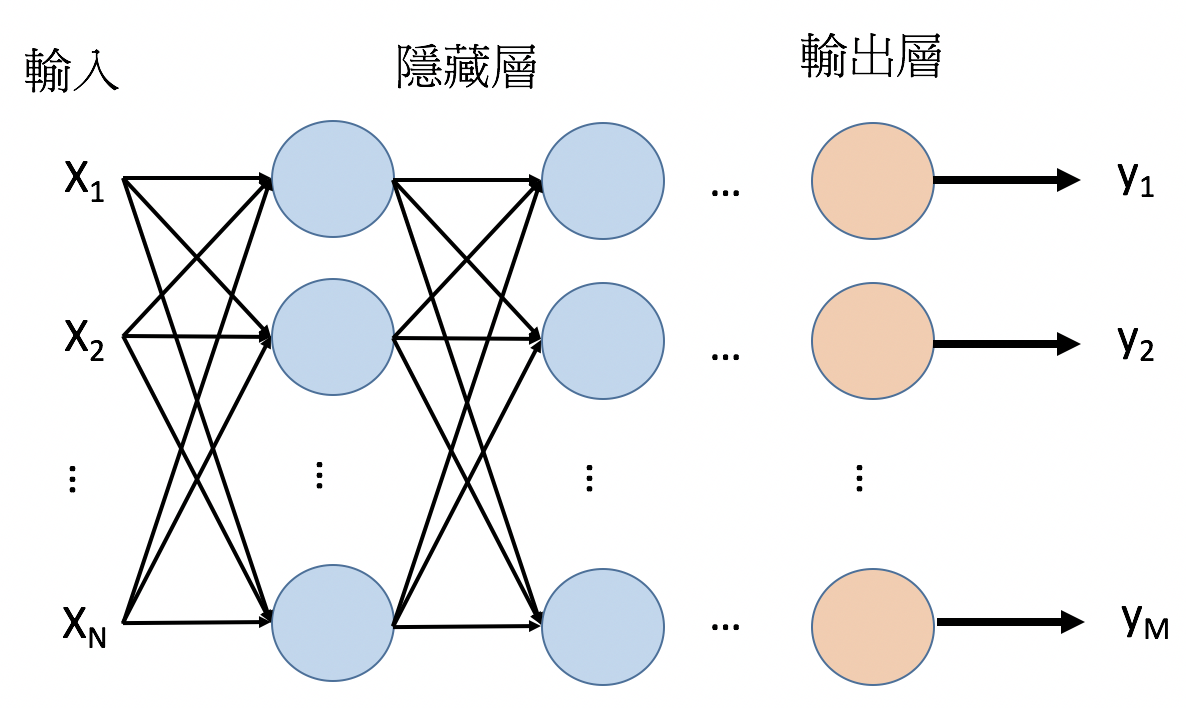
\includegraphics[scale=0.25]{images/ch2_DNN.png}\label{fig:ch2_DNN_no_drop}}
\subfloat[][隨機丟棄的DNN]{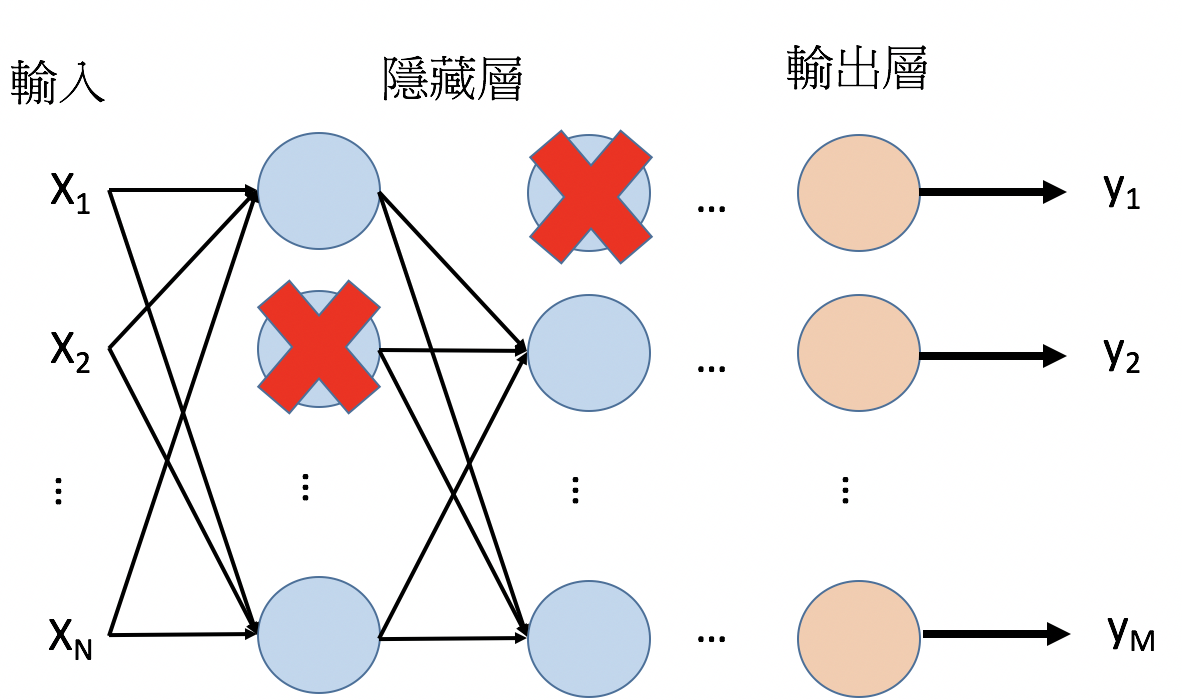
\includegraphics[scale=0.25]{images/ch2_dropout1.png}\label{fig:ch2_drop1}}
\subfloat[][隨機丟棄的DNN]{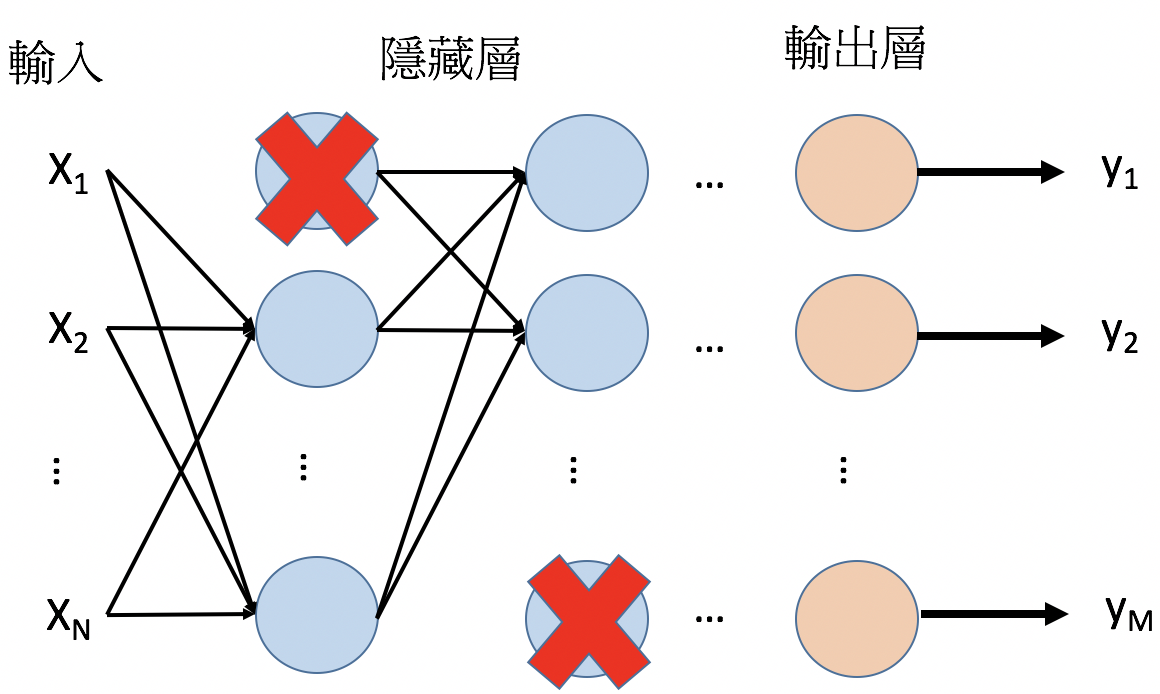
\includegraphics[scale=0.25]{images/ch2_dropout2.png}\label{fig:ch2_drop2}}
\caption{丟棄演算法}
\end{figure}
	丟棄演算法同時也可以視為隨機整合(Random Ensemble)模型。整合模型
	(Ensemble Model)在機器學習領域已經被證明是非常強大的模型,藉由多個模型的多樣性(Diversity)各司其職,提昇模型強度。類比在丟棄演算法中,根據不同的丟棄情況,有不同的神經元組合互相整合而成。隨機性造就了多樣性,又同時控制調適,使得模型更不容易過度貼合。

\end{itemize}
\section{遞迴式類神經網路(Recurrent Neural Network,RNN)}
\subsection{簡介}
類神經網絡已經是非常強大的模型,但對它而言,每次輸入都是獨立的,它並不記得曾經有過什麼樣的
輸入。這樣的類神經網絡對於有時序性(Sequential),且有上下文關係(Context
Dependency)的輸入時,例如語音辨識(Speech
Recognition)和自然語言理解(Naturl
Language Understanding),便無法表現得太好。因此讓類神經網路加上記憶的能力,即為遞迴式類神經網路(Recurrent
Neural Network)~\cite{elman1990finding}。

\begin{figure}[h]
\centering
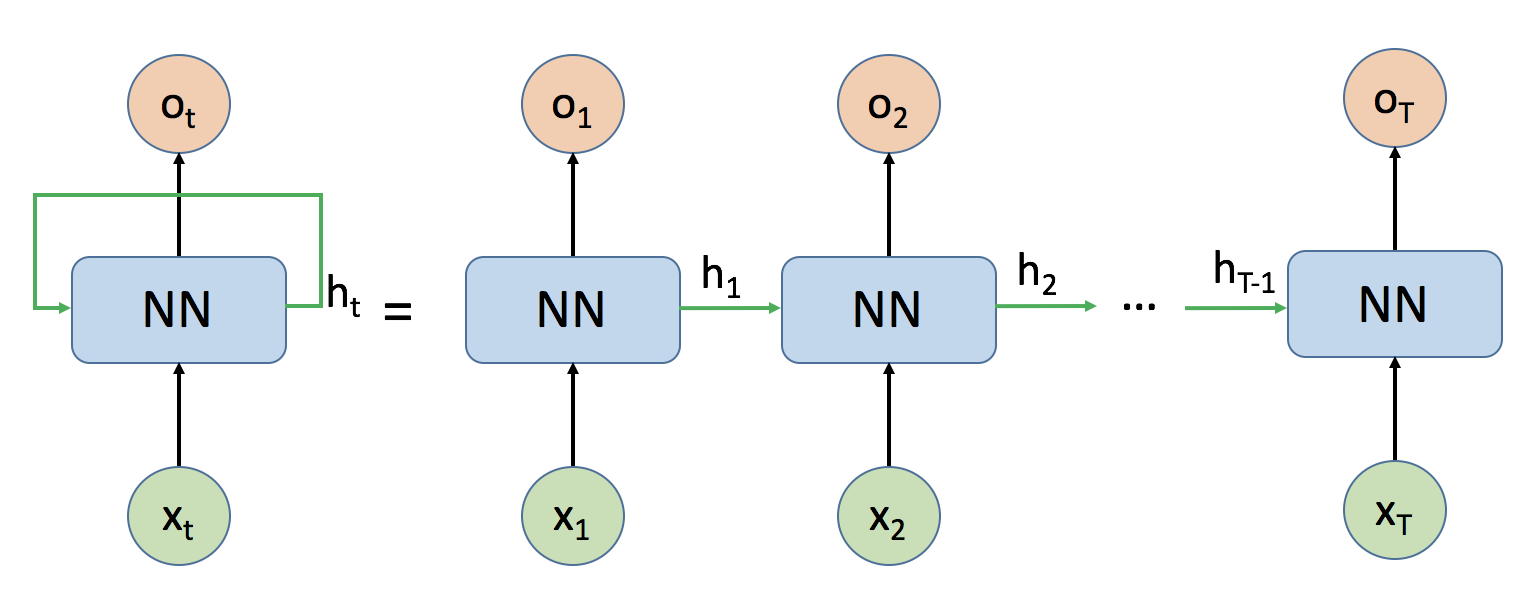
\includegraphics[scale=0.5]{images/ch2_RNN.png}
\caption{遞迴式類神經網路架構圖} \label{fig:ch2_RNN}
\end{figure}
\subsection{運作原理}
	圖~\ref{fig:ch2_RNN}為模型架構, $ NN $ 為一組類神經網路, $ x_t,o_t,h_t $ 為時間點t的輸入、輸出跟記憶。透過記憶細胞,類神經網路能夠將之前輸入的資訊往後傳遞,並且影響後面的輸出。如下式\ref{eq:h_t}。
\begin{equation}
\label{eq:h_t}
\begin{aligned}
&h_t = \phi_h{(W_h x_t+U_h h_{t-1}+b_h)}
\\
&o_t = \phi_o{(W_o h_t+b_o)}
\end{aligned}
\end{equation}
記憶 $ h_t $ 會跟時間  $ t $  的輸入  $ x_t $  與上個時間點的記憶  $ h_{t-1} $  影響。
其中 $ W_h,W_o,U_h,b_o,b_h $ 為遞迴式類神經網路的參數, $ \phi_h,\phi_o $ 為活化函數。



\subsection{沿時間反向傳播演算法}
沿時間反向傳播演算法 (back propagation through time)~\cite{werbos1990backpropagation}的概念跟反向傳播演算法類似,其唯一不同的是每個時間的梯度(Gradient)會沿著時間往前傳,如圖\ref{fig:ch2_BPTT}紅色的梯度和綠色的梯度都會一直往前傳,更新模型的參數。實務上,須根據所設定的展開時間層數,往前傳播,且訓練後個時間點的隱藏層與隱藏層間的權重矩陣將取平均,以讓個時間點的權重相同。
\begin{figure}[ht]
\centering
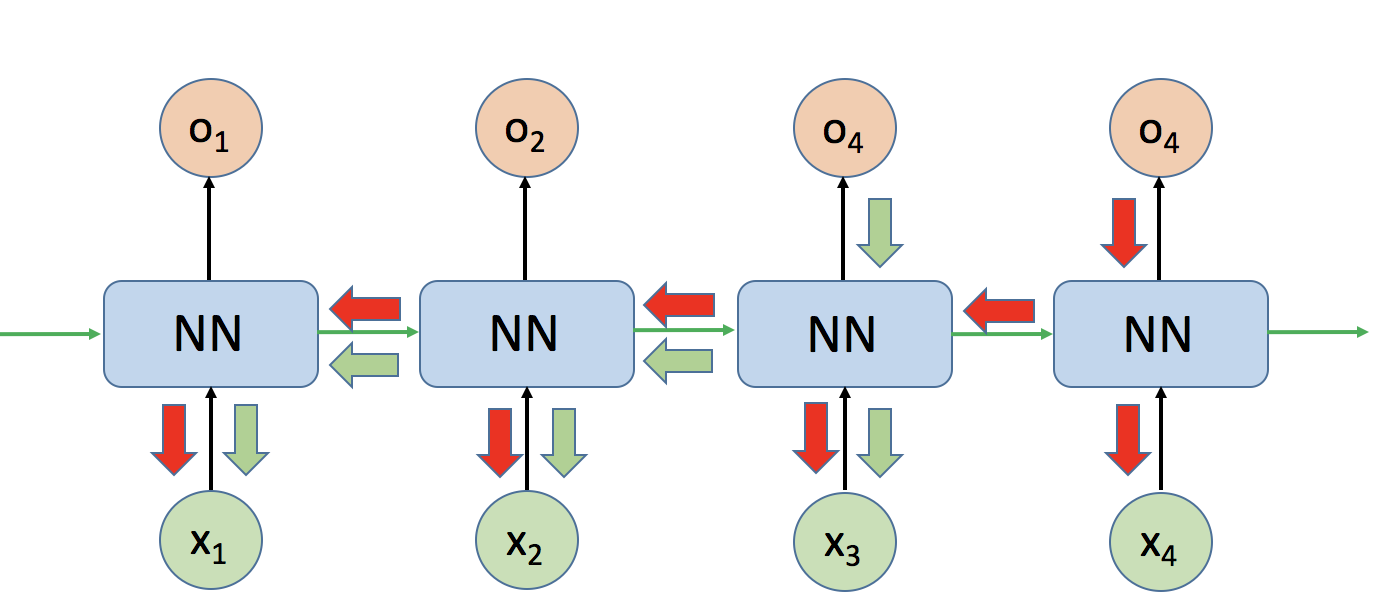
\includegraphics[scale=0.5]{images/ch2_BPTT.png}
\caption{沿時間反向傳播演算法的示意圖} \label{fig:ch2_BPTT}
\end{figure}

\subsection{長短期記憶神經網路}
\label{LSTM}
隨著輸入序列的長度加長,遞迴神經網路無法記得一開始的資訊,同時跟人類一樣,我們不需要記憶每個時間點的資訊,只需要記憶關鍵的資訊。因此更近一步提出一種進階形式:長短期記憶網路(Long Short-term Memory
Network)\cite{gers2001long},是一種特殊的遞迴神經網路,能夠彌補之前的缺點。
長短期記憶網路,比一般遞迴神經網路來得複雜,將原本的類神經元由長短期記憶細胞(Long
Short-term Memory Cell)取代,如圖\ref{fig:ch2_lstm},在每個時間點,這組神經網路會有一個單元狀態(Cell
State),並使用三個被稱作門限(Gate)的機制來輔助管理、移除、以及新增資訊。以下將會詳細說明各門限及其運作方式。
\begin{figure}[ht]
\centering
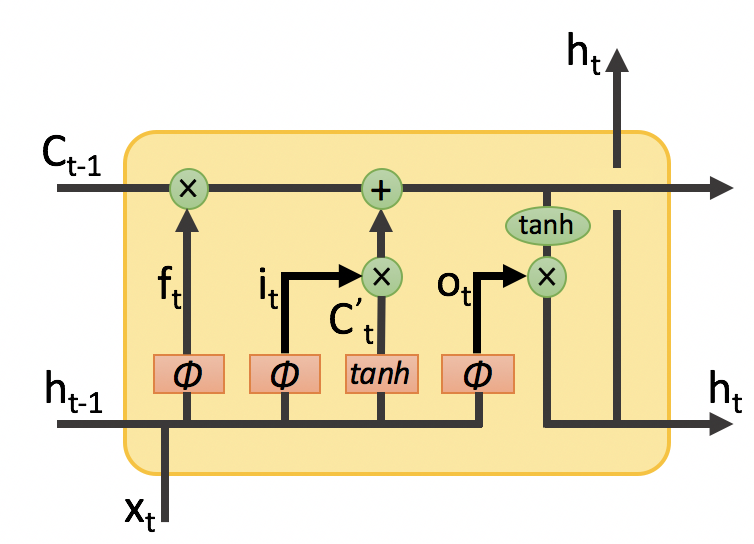
\includegraphics[scale=0.5]{images/ch2_lstm.png}
\caption{長短期記憶細胞的示意圖\cite{shen2016}} \label{fig:ch2_lstm}
\end{figure}
\begin{itemize}
\item{遺忘門限(Forget Gate) $ f_t $ }
	
	負責決定哪些資訊需要從單元狀態中丟棄。
	如式子\ref{eq:forget_gate}跟圖\ref{fig:ch2_forget_gate},依照前一個時序的輸出以及現在的輸入,產生一個值介於 $ 0 $ 到 $ 1 $ 的向量,藉由跟前一單元狀態 $ C_{t-1} $ 進行逐點乘積(Pointwise
	Product)時,可以決定哪些值要被捨棄多少。其中 $ \phi $ 表S型函數、 $ x_t $ 為第 $ t $ 個時刻的輸入、 $ h_{t-1} $ 則為前一時刻的輸出。
\begin{equation}
\label{eq:forget_gate}
f_t =  \phi( W_{xf} x_t + W_{hf} h_{t-1}+b_f)
\end{equation}
\begin{figure}[ht]
\centering
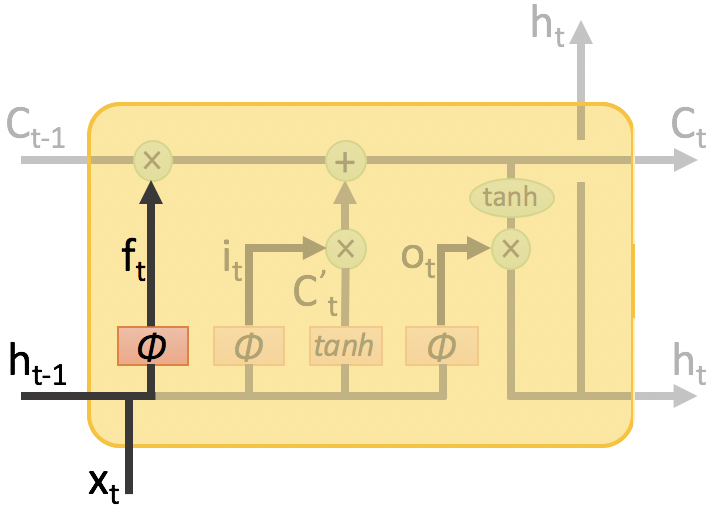
\includegraphics[scale=0.5]{images/ch2_forget_gate.png}
\caption{遺忘門限的運作圖\cite{shen2016}} \label{fig:ch2_forget_gate}
\end{figure}
\item{輸入門限(Input Gate) $ i_t $ } 

負責控制輸入訊息,假如模型認為是此時輸入為雜訊,可以將輸入門限設為0,反之設為1。另一個非線性函數雙曲正切(Hyperbolic
Tangent,tanh)將負責產生此時間點儲存資訊的候選值 $ C'_t $ 。如式\ref{eq:input_gate},圖\ref{fig:ch2_input_gate}所示。
\begin{equation}
\label{eq:input_gate}
\begin{aligned}
&i_t = \phi( W_{xi} x_t +W_{hi} h_{t-1} +b_i)
\\
&C'_i = tanh( W_{xC} x_t +W_{hC} h_{t-1} +b_C)
\end{aligned}
\end{equation}
\begin{figure}[ht]
\centering
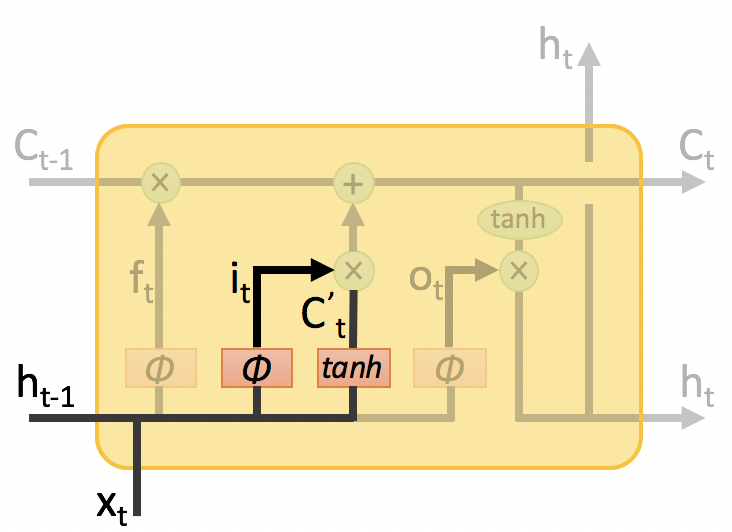
\includegraphics[scale=0.5]{images/ch2_input_gate.png}
\caption{輸入門限的運作圖\cite{shen2016}} \label{fig:ch2_input_gate}
\end{figure}
\item{更新單元狀態(Cell State)}

基於上面幾個運算,現在可以更新單元狀態,如式\ref{eq:update},圖\ref{fig:ch2_update}。新的單元狀態為上一個時間點的單元狀態 $ C_{t-1} $ 乘上遺忘門限 $ f_t $ 與此時的單元狀態候選 $ C'_t $ 乘上輸入門限 $ i_t $ 相加。
\begin{equation}
\label{eq:update}
C_t = f_t * C_{t-1} + i_t * C'_t
\end{equation}
\begin{figure}[ht]
\centering
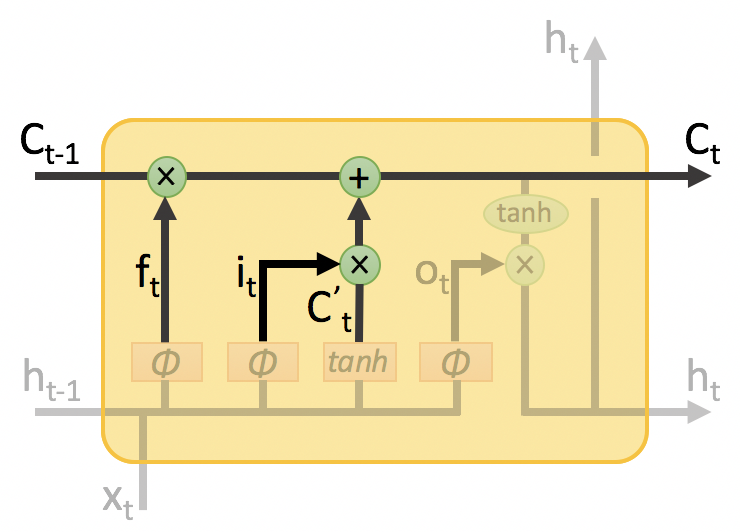
\includegraphics[scale=0.5]{images/ch2_update.png}
\caption{更新單元狀態的運作圖\cite{shen2016}} \label{fig:ch2_update}
\end{figure}
\item{輸出門限(Output Gate) $ o_t $ }

輸出門限 $ o_t $ 控制模型的輸出結果,其運作方式為與將通過雙曲正切函數的單元狀態 $ C_t $ 產生出 $ h_t $ ,進行逐點乘積,如此使模型能夠輸出想要的部分。如式\ref{eq:output_gate},圖\ref{fig:ch2_output_gate}所示。
\begin{equation}
\label{eq:output_gate}
	\begin{aligned}
		&o_t = \phi (W_{xo} x_t +W_{ho} h_{t-1} +b_o)
		\\
		&h_t = o_t * tanh(C_t)
	\end{aligned}
\end{equation}
\begin{figure}[ht]
\centering
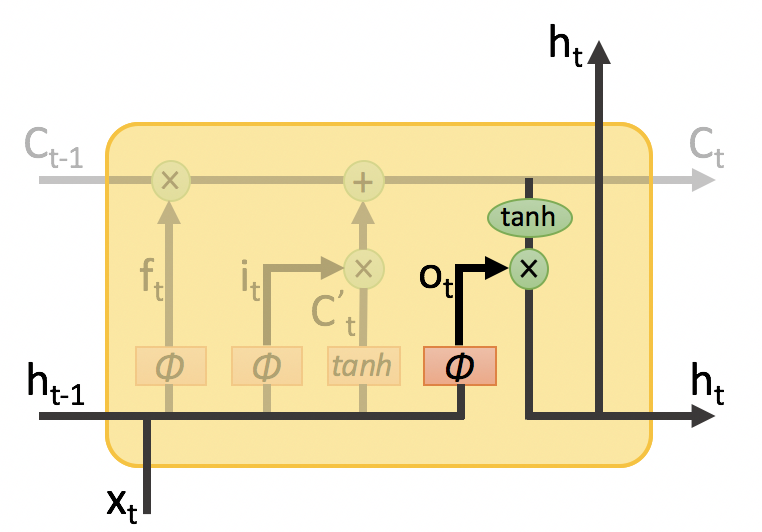
\includegraphics[scale=0.5]{images/ch2_output_gate.png}
\caption{輸出門限的運作圖\cite{shen2016}} \label{fig:ch2_output_gate}
\end{figure}
\end{itemize}

因上述的門限控制,可以使新的類神經網路,控制自己想要記憶的東西,而不是每個時間點的模型都會記憶下來,使其較久的資訊也能夠被模型記住。
\\
\\

\section{本章總結}
本章介紹了資訊檢索的背景,包含了基礎的資訊檢索架構、口述語彙偵測與語意檢索的差別,以及以動態時間校準做為口述語彙偵測的方法,再來介紹了類神經網路的基本原理,訓練方式及類神經網路常見的困難。最後介紹了遞迴式類神經網路,且介紹其中一種名為長短期記憶網路的運作方式。
